% P05 benchmark paired scatter; aggregate station-instrument domain means.
% Each point is a domain mean over common complete outer contexts; not an independent sample.
% data_sha256=235e8a7e1a4b0fc17b736ee7db3dcb16eaac30e233bc9eeb9ab4d033958dcc67
\documentclass[tikz,border=5pt]{standalone}
\ifdefined\pdfinfoomitdate\pdfinfoomitdate=1\fi
\ifdefined\pdfsuppressptexinfo\pdfsuppressptexinfo=-1\fi
\ifdefined\pdftrailerid\pdftrailerid{}\fi
\usepackage{pgfplots}
\usepgfplotslibrary{groupplots}
\pgfplotsset{compat=1.18}
\definecolor{p05Blue}{HTML}{0072B2}
\definecolor{p05Orange}{HTML}{E69F00}
\definecolor{p05Purple}{HTML}{CC79A7}
\begin{document}
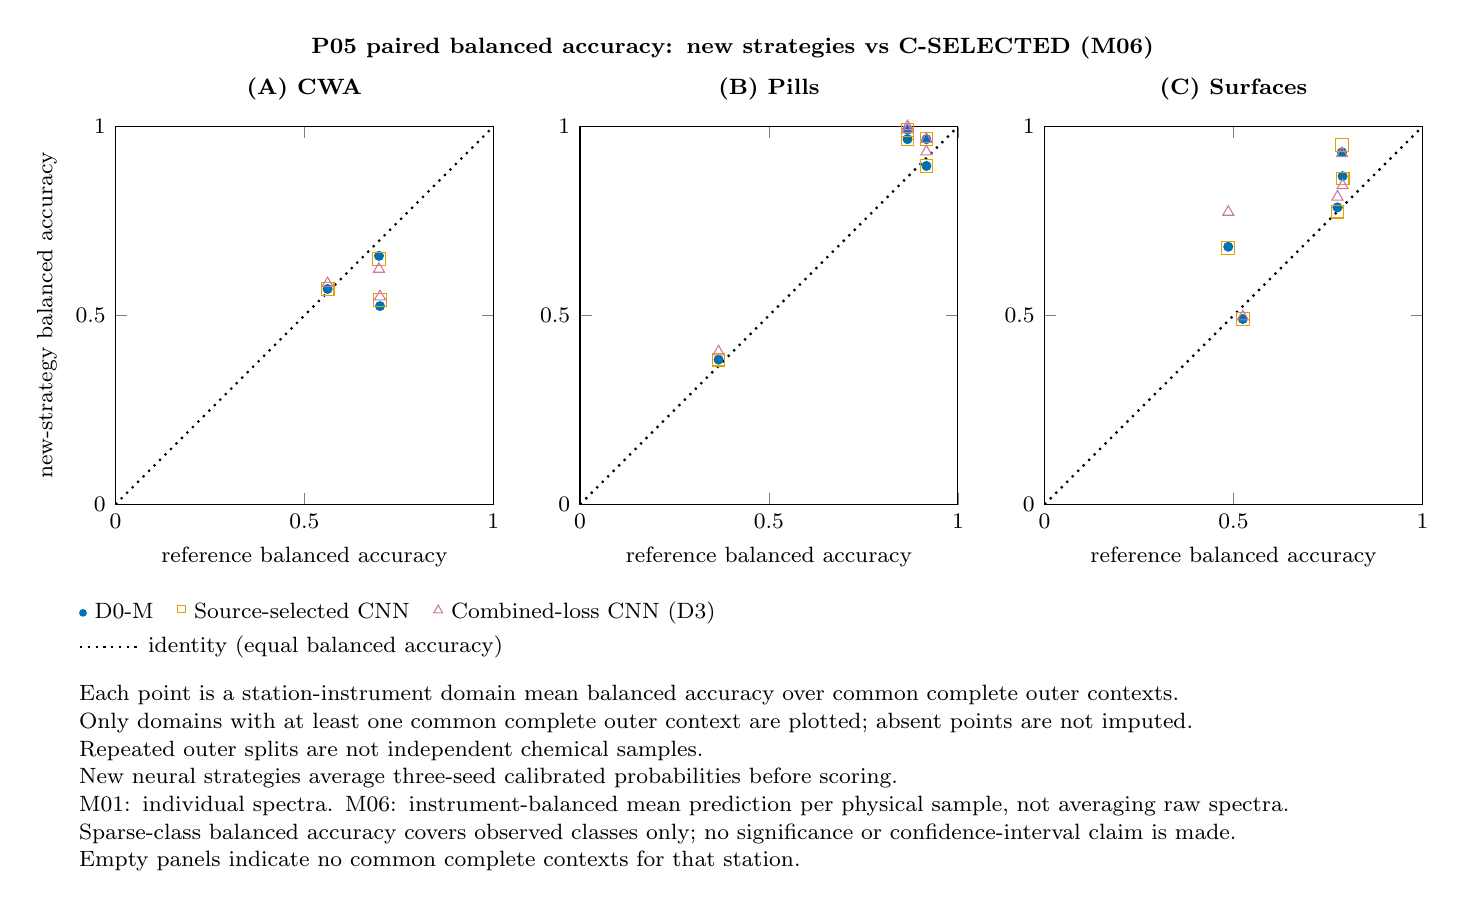
\begin{tikzpicture}
\begin{groupplot}[
  group style={group size=3 by 1, horizontal sep=1.1cm},
  width=4.8cm, height=4.8cm, scale only axis,
  xmin=0, xmax=1, ymin=0, ymax=1,
  xtick={0,0.5,1}, ytick={0,0.5,1},
  tick label style={font=\fontsize{8}{10}\selectfont, color=black},
  label style={font=\fontsize{8}{10}\selectfont, color=black},
  title style={font=\fontsize{8}{10}\selectfont\bfseries, color=black},
]
\nextgroupplot[title={(A) CWA}, xlabel={reference balanced accuracy}, ylabel={new-strategy balanced accuracy}]
\addplot[only marks, mark=*, mark size=1.6pt, color=p05Blue, mark options={fill=p05Blue, draw=p05Blue}] coordinates {(0.69999999999999996,0.52499999999999991) (0.56140350877192979,0.57017543859649111) (0.69736842105263153,0.6578947368421052)};
\addplot[only marks, mark=square, mark size=2.3pt, color=p05Orange, mark options={fill=none, draw=p05Orange}] coordinates {(0.69999999999999996,0.54166666666666663) (0.56140350877192979,0.57017543859649111) (0.69736842105263153,0.64912280701754388)};
\addplot[only marks, mark=triangle, mark size=2.3pt, color=p05Purple, mark options={fill=none, draw=p05Purple}] coordinates {(0.69999999999999996,0.54999999999999993) (0.56140350877192979,0.58479532163742687) (0.69736842105263153,0.62280701754385959)};
\addplot[black, dotted, line width=0.8pt] coordinates {(0,0) (1,1)};
\nextgroupplot[title={(B) Pills}, xlabel={reference balanced accuracy}]
\addplot[only marks, mark=*, mark size=1.6pt, color=p05Blue, mark options={fill=p05Blue, draw=p05Blue}] coordinates {(0.91666666666666663,0.89583333333333326) (0.91666666666666674,0.96666666666666656) (0.36666666666666659,0.38333333333333325) (0.86666666666666681,0.96666666666666656) (0.86666666666666681,0.99166666666666681)};
\addplot[only marks, mark=square, mark size=2.3pt, color=p05Orange, mark options={fill=none, draw=p05Orange}] coordinates {(0.91666666666666663,0.89583333333333326) (0.91666666666666674,0.96666666666666656) (0.36666666666666659,0.38333333333333325) (0.86666666666666681,0.96666666666666656) (0.86666666666666681,0.99166666666666681)};
\addplot[only marks, mark=triangle, mark size=2.3pt, color=p05Purple, mark options={fill=none, draw=p05Purple}] coordinates {(0.91666666666666663,0.93333333333333335) (0.91666666666666674,0.96666666666666656) (0.36666666666666659,0.40416666666666662) (0.86666666666666681,1) (0.86666666666666681,0.99166666666666681)};
\addplot[black, dotted, line width=0.8pt] coordinates {(0,0) (1,1)};
\nextgroupplot[title={(C) Surfaces}, xlabel={reference balanced accuracy}]
\addplot[only marks, mark=*, mark size=1.6pt, color=p05Blue, mark options={fill=p05Blue, draw=p05Blue}] coordinates {(0.52469135802469136,0.49074074074074076) (0.48611111111111105,0.68194444444444435) (0.78703703703703687,0.9320987654320988) (0.7885802469135802,0.86882716049382713) (0.77500000000000002,0.78611111111111109)};
\addplot[only marks, mark=square, mark size=2.3pt, color=p05Orange, mark options={fill=none, draw=p05Orange}] coordinates {(0.52469135802469136,0.49074074074074076) (0.48611111111111105,0.67916666666666659) (0.78703703703703687,0.95061728395061729) (0.7885802469135802,0.86265432098765427) (0.77500000000000002,0.77500000000000002)};
\addplot[only marks, mark=triangle, mark size=2.3pt, color=p05Purple, mark options={fill=none, draw=p05Purple}] coordinates {(0.52469135802469136,0.49691358024691357) (0.48611111111111105,0.77361111111111103) (0.78703703703703687,0.92901234567901225) (0.7885802469135802,0.84413580246913578) (0.77500000000000002,0.81388888888888877)};
\addplot[black, dotted, line width=0.8pt] coordinates {(0,0) (1,1)};
\end{groupplot}
\node[anchor=south, font=\fontsize{8}{10}\selectfont\bfseries, color=black, align=center, text width=16.6cm] at (current bounding box.north) {P05 paired balanced accuracy: new strategies vs C-SELECTED (M06)};
\node[anchor=north, font=\fontsize{8}{10}\selectfont, color=black, align=left, text width=16.6cm] (p05legend) at ([yshift=-2mm]current bounding box.south) {\tikz[baseline=-0.6ex]\fill[p05Blue](0,0)circle(1.4pt);\ D0-M\quad \tikz[baseline=-0.6ex]\draw[p05Orange](0,0)rectangle(2.8pt,2.8pt);\ Source-selected CNN\quad \tikz[baseline=-0.6ex]\draw[p05Purple](0,0)--(1.6pt,2.8pt)--(3.2pt,0)--cycle;\ Combined-loss CNN (D3)\\[0.8mm]\tikz[baseline=-0.6ex]\draw[black,dotted,line width=0.8pt](0,0)--(0.75,0);\ identity (equal balanced accuracy)};
\node[anchor=north, font=\fontsize{8}{10}\selectfont, color=black, align=left, text width=16.6cm] at ([yshift=-1mm]p05legend.south) {Each point is a station-instrument domain mean balanced accuracy over common complete outer contexts.\\Only domains with at least one common complete outer context are plotted; absent points are not imputed.\\Repeated outer splits are not independent chemical samples.\\New neural strategies average three-seed calibrated probabilities before scoring.\\M01: individual spectra. M06: instrument-balanced mean prediction per physical sample, not averaging raw spectra.\\Sparse-class balanced accuracy covers observed classes only; no significance or confidence-interval claim is made.\\Empty panels indicate no common complete contexts for that station.};
\end{tikzpicture}
\end{document}
